\begin{figure*}[hbtp]
  \centering
  \subfigure[Overall result]{
    \label{fig:8020-modularity--mean}
    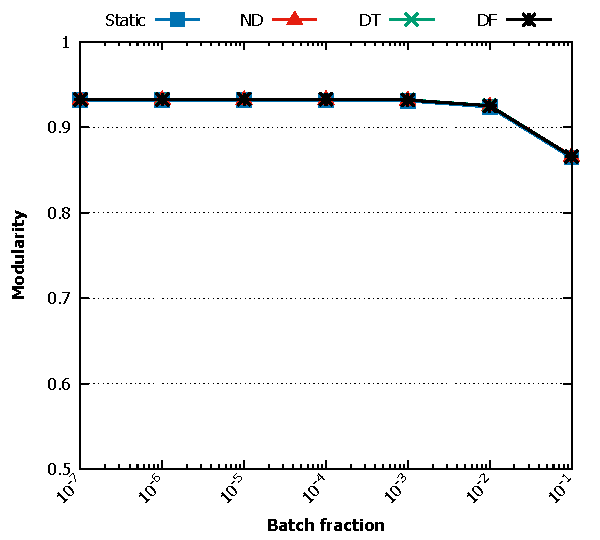
\includegraphics[width=0.38\linewidth]{out/8020-modularity-mean.pdf}
  }
  \subfigure[Results on each graph]{
    \label{fig:8020-modularity--all}
    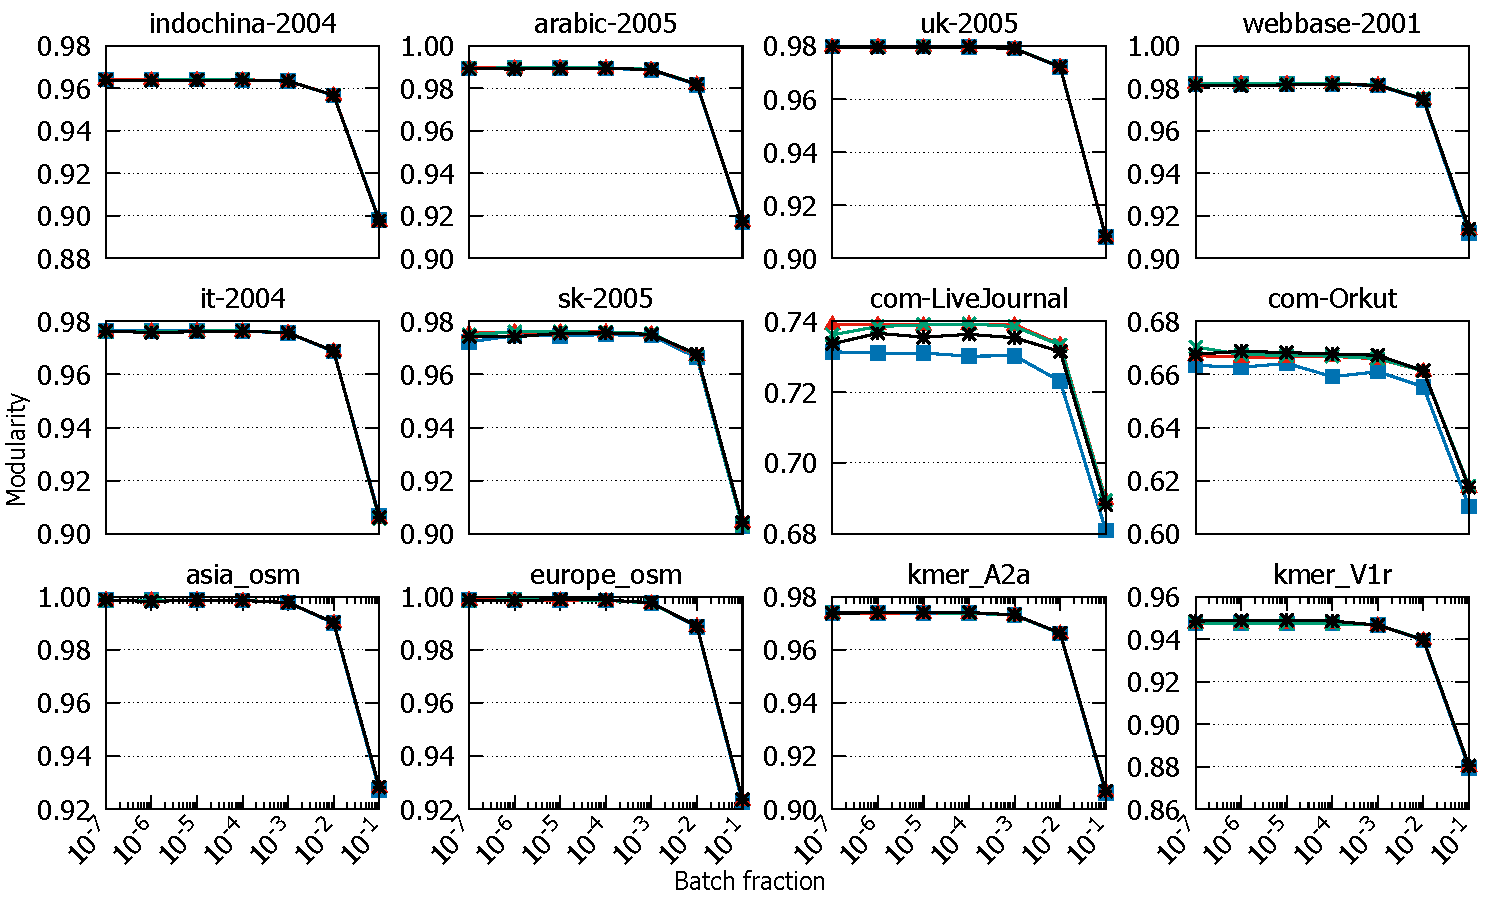
\includegraphics[width=0.58\linewidth]{out/8020-modularity-all.pdf}
  } \\[-2ex]
  \caption{Modularity comparison of our multicore implementation of \textit{Naive-dynamic (ND)}, \textit{Delta-screening (DS)}, and \textit{Dynamic Frontier (DF) Leiden}, compared to \textit{Static Leiden} \cite{sahu2024fast}, on large\ignore{(static)} graphs with randomly generated batch updates. These batch updates vary in size from $10^{-7}|E|$ to $0.1|E|$ in powers of 10, consisting of $80\%$ edge insertions and $20\%$ edge deletions to mimic realistic dynamic graph updates. Here, the right subfigure shows the modularity for each algorithm for individual graphs in the dataset, while the left subfigure displays overall modularity obtained using arithmetic mean.}
  \label{fig:8020-modularity}
\end{figure*}
